\documentclass[12pt,letterpaper]{article}

% Packages
\usepackage[utf8]{inputenc}
\usepackage[margin=1in]{geometry}
\usepackage{amsmath,amssymb,amsthm}
\usepackage{graphicx}
\usepackage{bm}
\usepackage{hyperref}
\usepackage{cite}
\usepackage{float}
\usepackage{enumitem}
\usepackage{algorithm}
\usepackage{algpseudocode}
\usepackage{siunitx}
\usepackage{tikz}
\usetikzlibrary{arrows.meta,positioning,calc,3d}

% Math commands
\newcommand{\vect}[1]{\bm{#1}}
\newcommand{\mat}[1]{\bm{#1}}
\newcommand{\deriv}[2]{\frac{d#1}{d#2}}
\newcommand{\pderiv}[2]{\frac{\partial #1}{\partial #2}}
\newcommand{\cross}{\times}

% Title
\title{\textbf{Simplified Six Degrees of Freedom Aircraft Dynamics:\\Mathematical Formulation and Implementation}}
\author{Technical Documentation}
\date{\today}

\begin{document}

\maketitle

\begin{abstract}
This document presents a comprehensive mathematical formulation of a simplified six degrees of freedom (6-DOF) rigid body dynamics model for fixed-wing aircraft. The model is designed for rapid prototyping, control system development, and reinforcement learning applications. We derive the complete equations of motion from first principles, discuss the aerodynamic theory underlying the force and moment models, analyze the assumptions and limitations, and provide implementation details including numerical integration strategies. The formulation strikes a balance between physical fidelity and computational efficiency, making it suitable for real-time simulation and iterative design workflows.
\end{abstract}

\tableofcontents
\newpage

% ============================================================================
\section{Introduction}
% ============================================================================

\subsection{Overview of 6-DOF Rigid Body Dynamics}

The motion of a rigid aircraft through three-dimensional space is characterized by six degrees of freedom: three translational coordinates defining the position of the center of mass, and three rotational coordinates defining the orientation of the aircraft-fixed body frame. The complete description of aircraft motion requires the solution of Newton's second law for translation and Euler's equations for rotational motion, both formulated in the body-fixed coordinate system where the inertia tensor is constant.

The 6-DOF equations of motion form the foundation of flight dynamics analysis and are essential for:
\begin{itemize}[noitemsep]
    \item Flight simulation and pilot training systems
    \item Control system design and validation
    \item Trajectory optimization and mission planning
    \item Stability and handling qualities analysis
    \item Reinforcement learning for autonomous flight
\end{itemize}

The full nonlinear 6-DOF equations capture the coupled nature of aircraft motion, where longitudinal and lateral-directional dynamics interact through kinematic and inertial coupling terms. This coupling is particularly significant during aggressive maneuvers or at high angles of attack.

\subsection{Applications in Flight Simulation and Control Systems}

Modern flight control system development relies heavily on high-fidelity simulations to validate algorithms before flight testing. The 6-DOF model serves as the "plant" in control system design, providing the necessary realism to test:
\begin{itemize}[noitemsep]
    \item Inner-loop attitude stabilization controllers (roll, pitch, yaw rate control)
    \item Outer-loop trajectory tracking controllers (altitude hold, heading hold, waypoint navigation)
    \item Adaptive and nonlinear control strategies
    \item Fault-tolerant control under actuator failures
\end{itemize}

For reinforcement learning applications, where thousands or millions of training episodes may be required, computational efficiency becomes paramount. Simplified models that capture the essential dynamics while omitting higher-order effects enable faster training without sacrificing the ability to learn meaningful control policies.

\subsection{Scope and Purpose of the Simplified Model}

This document describes a simplified 6-DOF model with the following characteristics:

\textbf{Included physics:}
\begin{itemize}[noitemsep]
    \item Rigid body translational and rotational dynamics
    \item Aerodynamic forces (lift, drag, side force) with linear coefficient models
    \item Aerodynamic moments (roll, pitch, yaw) including control derivatives and damping
    \item Thrust force aligned with body x-axis
    \item Gravitational force transformed to body frame
    \item Fourth-order Runge-Kutta numerical integration
\end{itemize}

\textbf{Simplifications and omissions:}
\begin{itemize}[noitemsep]
    \item Diagonal inertia tensor (product of inertia terms neglected)
    \item Flat Earth, non-rotating reference frame
    \item No propeller gyroscopic effects or slipstream
    \item No ground effect aerodynamics
    \item No atmospheric turbulence or wind (can be added as disturbances)
    \item Linear aerodynamic coefficient models (no stall modeling)
    \item No structural flexibility or aeroelastic effects
\end{itemize}

The model is calibrated for small fixed-wing aircraft (e.g., Cessna 172, large RC aircraft) with typical mass around 10 kg and wingspans of 2 meters. Parameter values are provided that yield realistic flight characteristics suitable for control system testing.

% ============================================================================
\section{Coordinate Systems and Frames of Reference}
% ============================================================================

\subsection{North-East-Down (NED) Inertial Frame}

The North-East-Down (NED) frame is an Earth-fixed inertial reference frame commonly used in aerospace applications. The origin is typically placed at a reference point on the Earth's surface (e.g., takeoff location), with axes defined as:
\begin{align}
\vect{x}_N &: \text{North direction (aligned with local geodetic north)} \\
\vect{y}_N &: \text{East direction (perpendicular to north, eastward)} \\
\vect{z}_N &: \text{Down direction (toward Earth's center, completing right-hand system)}
\end{align}

The aircraft position is denoted $\vect{r}^N = [x_N, y_N, z_N]^T$ in the NED frame. Altitude above ground level is $h = -z_N$ (negative because down is positive).

\textbf{Flat Earth assumption:} We treat the NED frame as inertial, neglecting Earth rotation ($\vect{\omega}_E \approx 7.29 \times 10^{-5}$ rad/s) and curvature. This is valid for flights of limited duration and range where Coriolis and centrifugal accelerations are negligible compared to gravitational and aerodynamic accelerations.

\subsection{Body-Fixed Coordinate System}

The body-fixed frame $F_B$ is rigidly attached to the aircraft with origin at the center of mass. The axes are defined according to aerospace convention:
\begin{align}
\vect{x}_B &: \text{Forward, through the nose (longitudinal axis)} \\
\vect{y}_B &: \text{Right wing direction (lateral axis)} \\
\vect{z}_B &: \text{Downward through the belly (vertical axis)}
\end{align}

The velocity of the aircraft center of mass expressed in the body frame is:
\begin{equation}
\vect{V}^B = [u, v, w]^T
\end{equation}
where $u$ is forward velocity, $v$ is lateral (sideslip) velocity, and $w$ is vertical velocity.

The angular velocity vector of the body frame relative to the inertial frame, expressed in body axes, is:
\begin{equation}
\vect{\omega}^B = [p, q, r]^T
\end{equation}
where $p$ is roll rate, $q$ is pitch rate, and $r$ is yaw rate.

\subsection{Transformation Between Frames}

The orientation of the body frame relative to the NED frame is parameterized by three Euler angles following the 3-2-1 (yaw-pitch-roll) rotation sequence:
\begin{align}
\phi &: \text{Roll angle (rotation about } \vect{x}_B \text{)} \\
\theta &: \text{Pitch angle (rotation about } \vect{y}_B \text{)} \\
\psi &: \text{Yaw angle (rotation about } \vect{z}_B \text{)}
\end{align}

The transformation from body frame to NED frame is accomplished by the direction cosine matrix (DCM):
\begin{equation}
\mat{R}^{NB}(\phi, \theta, \psi) = \mat{R}_3(\psi) \mat{R}_2(\theta) \mat{R}_1(\phi)
\label{eq:dcm}
\end{equation}

where the individual rotation matrices are:
\begin{align}
\mat{R}_1(\phi) &= \begin{bmatrix}
1 & 0 & 0 \\
0 & \cos\phi & -\sin\phi \\
0 & \sin\phi & \cos\phi
\end{bmatrix} \\
\mat{R}_2(\theta) &= \begin{bmatrix}
\cos\theta & 0 & \sin\theta \\
0 & 1 & 0 \\
-\sin\theta & 0 & \cos\theta
\end{bmatrix} \\
\mat{R}_3(\psi) &= \begin{bmatrix}
\cos\psi & -\sin\psi & 0 \\
\sin\psi & \cos\psi & 0 \\
0 & 0 & 1
\end{bmatrix}
\end{align}

Expanding Equation~\eqref{eq:dcm}, we obtain:
\begin{equation}
\mat{R}^{NB} = \begin{bmatrix}
\cos\theta\cos\psi & \sin\phi\sin\theta\cos\psi - \cos\phi\sin\psi & \cos\phi\sin\theta\cos\psi + \sin\phi\sin\psi \\
\cos\theta\sin\psi & \sin\phi\sin\theta\sin\psi + \cos\phi\cos\psi & \cos\phi\sin\theta\sin\psi - \sin\phi\cos\psi \\
-\sin\theta & \sin\phi\cos\theta & \cos\phi\cos\theta
\end{bmatrix}
\label{eq:dcm_full}
\end{equation}

A vector $\vect{v}^B$ in body coordinates is transformed to NED coordinates by:
\begin{equation}
\vect{v}^N = \mat{R}^{NB} \vect{v}^B
\end{equation}

The inverse transformation is simply the matrix transpose (since $\mat{R}^{NB}$ is orthogonal):
\begin{equation}
\vect{v}^B = (\mat{R}^{NB})^T \vect{v}^N = \mat{R}^{BN} \vect{v}^N
\end{equation}

\begin{figure}[H]
\centering
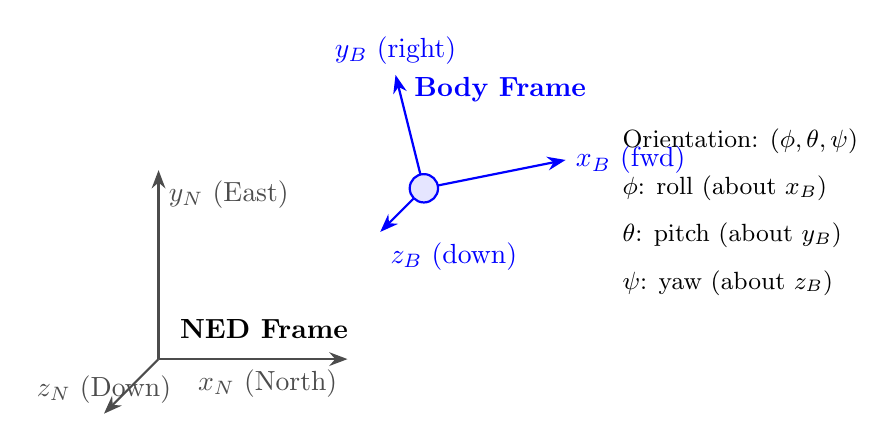
\begin{tikzpicture}[scale=1.2, >=Stealth]
    % NED frame
    \draw[->,thick,black!70] (0,0,0) -- (2,0,0) node[anchor=north east]{$x_N$ (North)};
    \draw[->,thick,black!70] (0,0,0) -- (0,2,0) node[anchor=north west]{$y_N$ (East)};
    \draw[->,thick,black!70] (0,0,0) -- (0,0,1.5) node[anchor=south]{$z_N$ (Down)};

    % Body frame (rotated)
    \coordinate (O) at (3,2,0.5);
    \draw[->,thick,blue] (O) -- ++(1.5,0.3,0) node[anchor=west]{$x_B$ (fwd)};
    \draw[->,thick,blue] (O) -- ++(-0.3,1.2,0) node[anchor=south]{$y_B$ (right)};
    \draw[->,thick,blue] (O) -- ++(0,0,1.2) node[anchor=north west]{$z_B$ (down)};

    % Aircraft symbol
    \draw[thick,blue,fill=blue!10] (O) circle (0.15);

    % Labels
    \node[anchor=south] at (1,0,-0.3) {\textbf{NED Frame}};
    \node[anchor=south,blue] at (3.5,2.5,-0.3) {\textbf{Body Frame}};

    % Euler angle annotations
    \node[anchor=west,font=\small] at (5,2.5,0.5) {Orientation: $(\phi, \theta, \psi)$};
    \node[anchor=west,font=\small] at (5,2,0.5) {$\phi$: roll (about $x_B$)};
    \node[anchor=west,font=\small] at (5,1.5,0.5) {$\theta$: pitch (about $y_B$)};
    \node[anchor=west,font=\small] at (5,1,0.5) {$\psi$: yaw (about $z_B$)};
\end{tikzpicture}
\caption{NED inertial frame and body-fixed coordinate frame. The body frame orientation relative to NED is parameterized by Euler angles $(\phi, \theta, \psi)$ using a 3-2-1 rotation sequence.}
\label{fig:coordinate_frames}
\end{figure}

\subsection{Euler Angles and Their Limitations}

Euler angles provide an intuitive parameterization of orientation but suffer from a critical limitation: \textbf{gimbal lock}. This singularity occurs when the pitch angle approaches $\theta = \pm 90°$, causing the roll and yaw axes to align. At this configuration, the transformation between Euler rates and body angular rates becomes undefined (division by $\cos\theta = 0$).

\textbf{Mitigation strategies:}
\begin{enumerate}[noitemsep]
    \item \textbf{Clamping:} Restrict pitch angle to safe range, e.g., $\theta \in [-85°, +85°]$ (implemented in this model)
    \item \textbf{Quaternion representation:} Use unit quaternions to avoid singularities (not used here for simplicity)
    \item \textbf{Alternative Euler sequences:} Different rotation sequences have singularities at different orientations
\end{enumerate}

For typical aircraft operations (excluding aerobatics), pitch angles rarely exceed $\pm 30°$, making Euler angles acceptable. The pitch clamping in our implementation provides robust protection against numerical issues.

% ============================================================================
\section{Mathematical Formulation}
% ============================================================================

\subsection{Kinematic Equations}

Kinematics relates the time derivatives of position and orientation to the velocity and angular rates. These equations do not involve forces or dynamics; they are purely geometric relationships.

\subsubsection{Position Derivatives}

The position of the aircraft in the NED frame evolves according to the velocity vector. However, the velocity is most naturally expressed in the body frame (where aerodynamic forces act). The position derivative is:
\begin{equation}
\dot{\vect{r}}^N = \mat{R}^{NB} \vect{V}^B
\label{eq:pos_dot}
\end{equation}

Expanding using Equation~\eqref{eq:dcm_full}:
\begin{align}
\dot{x}_N &= u\cos\theta\cos\psi + v(\sin\phi\sin\theta\cos\psi - \cos\phi\sin\psi) \nonumber \\
&\quad + w(\cos\phi\sin\theta\cos\psi + \sin\phi\sin\psi) \\
\dot{y}_N &= u\cos\theta\sin\psi + v(\sin\phi\sin\theta\sin\psi + \cos\phi\cos\psi) \nonumber \\
&\quad + w(\cos\phi\sin\theta\sin\psi - \sin\phi\cos\psi) \\
\dot{z}_N &= -u\sin\theta + v\sin\phi\cos\theta + w\cos\phi\cos\theta
\label{eq:pos_dot_expanded}
\end{align}

\textbf{Physical interpretation:} The body frame velocity components $(u, v, w)$ are projected onto the NED axes through the rotation matrix, accounting for the aircraft's current orientation. For example, a purely forward velocity $u$ in level flight ($\phi = \theta = 0$) contributes to north and east velocity according to the heading $\psi$.

\subsubsection{Euler Angle Rate Equations}

The relationship between body angular rates $\vect{\omega}^B = [p, q, r]^T$ and Euler angle rates $[\dot{\phi}, \dot{\theta}, \dot{\psi}]^T$ is derived from the kinematic constraint that the body angular velocity can be decomposed into contributions from each Euler rate.

The Euler angle rates transform to body rates through:
\begin{equation}
\vect{\omega}^B = \begin{bmatrix} p \\ q \\ r \end{bmatrix} =
\begin{bmatrix}
1 & 0 & -\sin\theta \\
0 & \cos\phi & \sin\phi\cos\theta \\
0 & -\sin\phi & \cos\phi\cos\theta
\end{bmatrix}
\begin{bmatrix} \dot{\phi} \\ \dot{\theta} \\ \dot{\psi} \end{bmatrix}
\label{eq:euler_to_body}
\end{equation}

Inverting this relationship yields the Euler angle rates:
\begin{equation}
\begin{bmatrix} \dot{\phi} \\ \dot{\theta} \\ \dot{\psi} \end{bmatrix} =
\begin{bmatrix}
1 & \sin\phi\tan\theta & \cos\phi\tan\theta \\
0 & \cos\phi & -\sin\phi \\
0 & \sin\phi/\cos\theta & \cos\phi/\cos\theta
\end{bmatrix}
\begin{bmatrix} p \\ q \\ r \end{bmatrix}
\label{eq:euler_rates}
\end{equation}

Explicitly:
\begin{align}
\dot{\phi} &= p + q\sin\phi\tan\theta + r\cos\phi\tan\theta \label{eq:phi_dot} \\
\dot{\theta} &= q\cos\phi - r\sin\phi \label{eq:theta_dot} \\
\dot{\psi} &= \frac{q\sin\phi + r\cos\phi}{\cos\theta} \label{eq:psi_dot}
\end{align}

\textbf{Physical interpretation:}
\begin{itemize}[noitemsep]
    \item Roll rate $p$ directly contributes to $\dot{\phi}$, but also induces yaw and pitch rate changes due to orientation
    \item Pitch rate $q$ directly affects $\dot{\theta}$ (modified by roll angle)
    \item Yaw rate $r$ couples into all three Euler rates, with magnitude depending on pitch and roll
\end{itemize}

\subsubsection{Gimbal Lock Singularity}

Equations~\eqref{eq:phi_dot}--\eqref{eq:psi_dot} contain terms with $\tan\theta$ and $1/\cos\theta$, which become infinite as $\theta \to \pm 90°$. This is the gimbal lock singularity.

\textbf{Implementation mitigation:} To prevent numerical overflow at the singularity, we clamp $\theta$ to a safe range during integration:
\begin{equation}
\theta_{\text{safe}} = \text{clamp}(\theta, -85°, +85°)
\end{equation}

\textbf{Important caveat:} Clamping prevents the \textit{numerical singularity} (division by $\cos\theta = 0$) but does not prevent \textit{gimbal lock behavior}. Near $\theta = 85°$:
\begin{itemize}[noitemsep]
    \item $\tan(85°) \approx 11.4$: Small errors in $q$ or $r$ are amplified 11$\times$ in $\dot{\phi}$ and $\dot{\psi}$ (see Eq.~\eqref{eq:euler_rates})
    \item Numerical conditioning degrades: Round-off errors accumulate rapidly
    \item Roll ($\phi$) and yaw ($\psi$) become nearly indistinguishable (loss of representational uniqueness)
\end{itemize}

\textbf{Recommendation:} For maneuvers exceeding $|\theta| > 60°$ (steep climbs/dives), or any sustained near-vertical flight, use quaternion attitude representation to avoid these issues entirely.

Additionally, Euler angles are wrapped to their principal ranges after each integration step:
\begin{align}
\phi &\in [-\pi, \pi] \\
\theta &\in [-85° \times \pi/180, +85° \times \pi/180] \\
\psi &\in [-\pi, \pi]
\end{align}

Wrapping for roll and yaw is accomplished via:
\begin{equation}
\text{wrap}(\alpha) = \text{atan2}(\sin\alpha, \cos\alpha)
\end{equation}
which maps any angle to $[-\pi, \pi]$.

% ============================================================================
\subsection{Dynamic Equations}
% ============================================================================

\subsubsection{Translational Dynamics: Newton's Second Law in Body Frame}

Newton's second law in an inertial frame states:
\begin{equation}
\vect{F} = m\ddot{\vect{r}}^N
\end{equation}

However, forces acting on the aircraft (aerodynamic, thrust) are most naturally expressed in the body frame. To formulate dynamics in body coordinates, we must account for the rotating reference frame.

The acceleration of the aircraft in the inertial frame can be related to the body frame by:
\begin{equation}
\left(\deriv{\vect{V}}{t}\right)^N = \left(\deriv{\vect{V}}{t}\right)^B + \vect{\omega}^B \cross \vect{V}^B
\end{equation}

Expressing Newton's law in body coordinates:
\begin{equation}
\vect{F}^B = m\left[\left(\deriv{\vect{V}^B}{t}\right) + \vect{\omega}^B \cross \vect{V}^B\right]
\label{eq:newton_body}
\end{equation}

The term $\vect{\omega}^B \cross \vect{V}^B$ represents the Coriolis and centrifugal accelerations due to the rotating body frame. Expanding the cross product:
\begin{equation}
\vect{\omega}^B \cross \vect{V}^B = \begin{bmatrix} p \\ q \\ r \end{bmatrix} \cross \begin{bmatrix} u \\ v \\ w \end{bmatrix} = \begin{bmatrix}
qw - rv \\
ru - pw \\
pv - qu
\end{bmatrix}
\end{equation}

Thus, the translational equations of motion in body coordinates are:
\begin{align}
\dot{u} &= \frac{F_x}{m} - qw + rv \label{eq:u_dot} \\
\dot{v} &= \frac{F_y}{m} - ru + pw \label{eq:v_dot} \\
\dot{w} &= \frac{F_z}{m} - pv + qu \label{eq:w_dot}
\end{align}

where $\vect{F}^B = [F_x, F_y, F_z]^T$ is the total force vector (aerodynamic + thrust + gravity) expressed in body axes.

\textbf{Physical interpretation:}
\begin{itemize}[noitemsep]
    \item The terms $F_x/m$, $F_y/m$, $F_z/m$ are the accelerations due to applied forces
    \item The cross-product terms ($qw - rv$, etc.) are fictitious accelerations arising from the rotating reference frame
    \item For example, in a coordinated turn with yaw rate $r$ and forward velocity $u$, the term $ru$ in Equation~\eqref{eq:v_dot} represents centrifugal acceleration pushing the aircraft outward
\end{itemize}

\subsubsection{Rotational Dynamics: Euler's Equations}

The rotational analog of Newton's second law relates the moment (torque) to angular acceleration. In body coordinates, Euler's equations for a rigid body are \cite{stevens2015, etkin2005}:
\begin{equation}
\vect{M}^B = \mat{I}\dot{\vect{\omega}}^B + \vect{\omega}^B \cross (\mat{I}\vect{\omega}^B)
\label{eq:euler_moments}
\end{equation}

where $\vect{M}^B = [L, M, N]^T$ is the moment vector (roll moment, pitch moment, yaw moment) and $\mat{I}$ is the inertia tensor.

For a general rigid body, the inertia tensor is:
\begin{equation}
\mat{I} = \begin{bmatrix}
I_{xx} & -I_{xy} & -I_{xz} \\
-I_{xy} & I_{yy} & -I_{yz} \\
-I_{xz} & -I_{yz} & I_{zz}
\end{bmatrix}
\end{equation}

\textbf{Diagonal inertia assumption:} We assume the body axes are aligned with the principal axes of inertia, so the products of inertia vanish:
\begin{equation}
I_{xy} = I_{xz} = I_{yz} = 0
\end{equation}

This simplification is excellent for symmetric aircraft and simplifies the equations considerably. The inertia tensor becomes:
\begin{equation}
\mat{I} = \begin{bmatrix}
I_{xx} & 0 & 0 \\
0 & I_{yy} & 0 \\
0 & 0 & I_{zz}
\end{bmatrix}
\end{equation}

Substituting into Equation~\eqref{eq:euler_moments} and expanding:
\begin{align}
L &= I_{xx}\dot{p} + (I_{zz} - I_{yy})qr \label{eq:L_moment} \\
M &= I_{yy}\dot{q} + (I_{xx} - I_{zz})pr \label{eq:M_moment} \\
N &= I_{zz}\dot{r} + (I_{yy} - I_{xx})pq \label{eq:N_moment}
\end{align}

Solving for angular accelerations:
\begin{align}
\dot{p} &= \frac{L - (I_{zz} - I_{yy})qr}{I_{xx}} \label{eq:p_dot} \\
\dot{q} &= \frac{M - (I_{xx} - I_{zz})pr}{I_{yy}} \label{eq:q_dot} \\
\dot{r} &= \frac{N - (I_{yy} - I_{xx})pq}{I_{zz}} \label{eq:r_dot}
\end{align}

\textbf{Gyroscopic coupling in the simplified implementation:}

\textbf{Important clarification:} The diagonal inertia assumption (products of inertia $I_{xy} = I_{xz} = I_{yz} = 0$) does NOT eliminate the gyroscopic coupling terms $(I_{zz} - I_{yy})qr$, $(I_{xx} - I_{zz})pr$, and $(I_{yy} - I_{xx})pq$ in Equations~\eqref{eq:p_dot}--\eqref{eq:r_dot}. These terms arise from the cross product $\vect{\omega}^B \cross (\mat{I}\vect{\omega}^B)$, not from off-diagonal inertia elements.

However, for our simplified implementation, we \textit{additionally} neglect these gyroscopic coupling terms, reducing to:
\begin{align}
\dot{p} &= \frac{L}{I_{xx}} \label{eq:p_dot_simple} \\
\dot{q} &= \frac{M}{I_{yy}} \label{eq:q_dot_simple} \\
\dot{r} &= \frac{N}{I_{zz}} \label{eq:r_dot_simple}
\end{align}

\textbf{Validity of this approximation:} The gyroscopic coupling terms are negligible when:
\begin{itemize}[noitemsep]
    \item Inertia ratios are near unity: $|I_{yy} - I_{zz}| \ll I_{xx}$, $|I_{xx} - I_{zz}| \ll I_{yy}$, etc.
    \item Angular rates are small: $p, q, r \ll \sqrt{L_{\max}/I_{xx}}$ (rates much smaller than maximum achievable)
    \item Aircraft has near-symmetric mass distribution (typical for fixed-wing aircraft)
\end{itemize}

For high-rate aerobatic maneuvers (coordinated loops, barrel rolls) or aircraft with large inertia asymmetry, the full coupled equations~\eqref{eq:p_dot}--\eqref{eq:r_dot} should be used.

\textbf{Physical interpretation:}
\begin{itemize}[noitemsep]
    \item Moments cause angular accelerations inversely proportional to moment of inertia (rotational analog of $F = ma$)
    \item The gyroscopic terms represent inertial coupling: a pitch rate $q$ combined with yaw rate $r$ induces a roll moment proportional to the difference in pitch and yaw inertias
    \item For symmetric aircraft, cross-coupling is primarily through aerodynamic effects, not inertial effects
\end{itemize}

% ============================================================================
\subsection{Forces}
% ============================================================================

The total force vector in body coordinates is the sum of aerodynamic, thrust, and gravitational contributions:
\begin{equation}
\vect{F}^B = \vect{F}_{\text{aero}}^B + \vect{F}_{\text{thrust}}^B + \vect{F}_{\text{grav}}^B
\end{equation}

\begin{figure}[H]
\centering
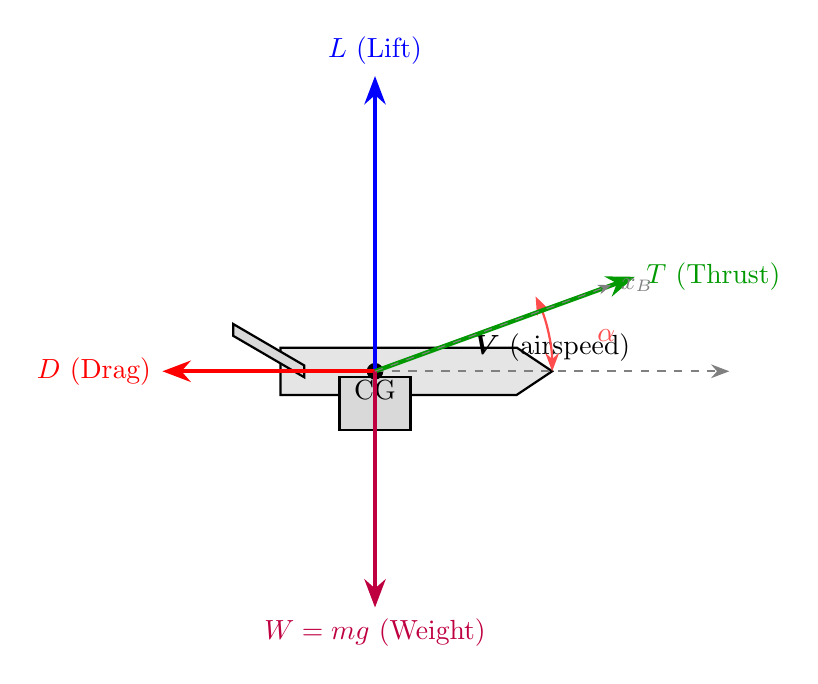
\begin{tikzpicture}[scale=1.5, >=Stealth]
    % Aircraft body (simplified side view)
    \coordinate (cg) at (0,0);
    \draw[thick,fill=gray!20] (-0.8,-0.2) -- (1.2,-0.2) -- (1.5,0) -- (1.2,0.2) -- (-0.8,0.2) -- cycle;
    \draw[thick,fill=gray!30] (-0.6,-0.05) -- (-0.6,0.05) -- (-1.2,0.4) -- (-1.2,0.3) -- cycle; % tail
    \draw[thick,fill=gray!30] (-0.3,-0.5) -- (-0.3,-0.05) -- (0.3,-0.05) -- (0.3,-0.5) -- cycle; % wing

    % Center of gravity marker
    \fill (cg) circle (2pt);
    \node[anchor=north] at (cg) {CG};

    % Velocity vector (reference)
    \draw[->,thick,gray,dashed] (cg) -- ++(3,0) node[midway,above,black] {$\vect{V}$ (airspeed)};

    % Angle of attack
    \draw[<->,thick,red!70] (1.5,0) arc[start angle=0, end angle=25, radius=1.5];
    \node[red!70,anchor=west] at (1.8,0.3) {$\alpha$};

    % Forces
    % Lift (perpendicular to velocity)
    \draw[->,ultra thick,blue] (cg) -- ++(0,2.5) node[anchor=south] {$L$ (Lift)};

    % Drag (parallel to velocity, opposing)
    \draw[->,ultra thick,red] (cg) -- ++(-1.8,0) node[anchor=east] {$D$ (Drag)};

    % Thrust (along body x-axis, approximately)
    \draw[->,ultra thick,green!60!black] (cg) -- ++(2.2,0.8) node[anchor=west] {$T$ (Thrust)};

    % Weight (downward in NED frame)
    \draw[->,ultra thick,purple] (cg) -- ++(0,-2) node[anchor=north] {$W = mg$ (Weight)};

    % Body axis (for reference)
    \draw[->,dashed,black!50] (cg) -- ++(2,0.73) node[anchor=west,font=\small] {$x_B$};

\end{tikzpicture}
\caption{Free-body diagram showing forces acting on the aircraft. Lift $L$ and drag $D$ are defined in the wind frame (relative to airspeed $\vect{V}$), thrust $T$ acts approximately along the body $x$-axis, and weight $W$ acts downward in the NED frame. Angle of attack $\alpha$ is the angle between the body $x$-axis and the velocity vector.}
\label{fig:free_body}
\end{figure}

\subsubsection{Aerodynamic Forces}

Aerodynamic forces arise from the pressure distribution over the aircraft surface as it moves through the air. These are typically decomposed into:
\begin{itemize}[noitemsep]
    \item \textbf{Lift} $L$: Force perpendicular to the relative wind (opposing gravity in steady level flight)
    \item \textbf{Drag} $D$: Force parallel to the relative wind, opposing motion
    \item \textbf{Side force} $Y$: Lateral force (typically small for symmetric aircraft in coordinated flight)
\end{itemize}

The magnitude of each force is given by:
\begin{align}
L &= q_{\infty} S C_L \label{eq:lift} \\
D &= q_{\infty} S C_D \label{eq:drag} \\
Y &= q_{\infty} S C_Y \label{eq:side_force}
\end{align}

where:
\begin{itemize}[noitemsep]
    \item $q_{\infty} = \frac{1}{2}\rho V^2$ is the dynamic pressure
    \item $\rho$ is air density (\SI{1.225}{kg/m^3} at sea level)
    \item $V$ is airspeed (magnitude of velocity: $V = \sqrt{u^2 + v^2 + w^2}$)
    \item $S$ is wing reference area
    \item $C_L, C_D, C_Y$ are dimensionless aerodynamic coefficients (discussed in Section 4)
\end{itemize}

\textbf{Transformation to body axes:}
Lift and drag are defined in the wind frame (aligned with relative wind). To transform to body axes, we use angle of attack $\alpha$ and sideslip angle $\beta$:
\begin{align}
\alpha &= \arctan\left(\frac{w}{u}\right) \label{eq:alpha} \\
\beta &= \arcsin\left(\frac{v}{V}\right) \label{eq:beta}
\end{align}

Assuming small sideslip ($\beta \approx 0$ for symmetric flight), the aerodynamic forces in body coordinates are:
\begin{align}
F_{x,\text{aero}} &= -D\cos\alpha + L\sin\alpha \label{eq:fx_aero} \\
F_{y,\text{aero}} &= Y \label{eq:fy_aero} \\
F_{z,\text{aero}} &= -D\sin\alpha - L\cos\alpha \label{eq:fz_aero}
\end{align}

\textbf{Physical interpretation:}
\begin{itemize}[noitemsep]
    \item At zero angle of attack ($\alpha = 0$), lift acts purely in the $-z_B$ direction (upward in body frame)
    \item Drag always opposes the velocity vector
    \item For small $\alpha$: $\cos\alpha \approx 1$, $\sin\alpha \approx \alpha$, so lift is primarily vertical and drag is primarily axial
    \item At high $\alpha$, lift rotates forward (contributing to $F_x$), which can reduce effective thrust
\end{itemize}

\subsubsection{Thrust Model}

Thrust is modeled as a force aligned with the body $x$-axis (forward direction), controlled by throttle $\delta_t \in [0, 1]$:
\begin{align}
F_{x,\text{thrust}} &= T_{\max} \delta_t \label{eq:thrust_x} \\
F_{y,\text{thrust}} &= 0 \\
F_{z,\text{thrust}} &= 0
\end{align}

where $T_{\max}$ is maximum thrust (e.g., \SI{50}{N} for a typical RC aircraft).

\textbf{Simplifications:}
\begin{itemize}[noitemsep]
    \item No thrust variation with airspeed (jet/prop thrust decreases with velocity)
    \item No propeller slipstream effects on wing/tail
    \item No gyroscopic moments from spinning propeller
    \item Thrust vector aligned with $x_B$ (no thrust vectoring or downwash angle)
\end{itemize}

\textbf{Important note on propeller thrust:}

The constant-thrust model is appropriate for \textit{jet aircraft}, where thrust is nearly independent of airspeed. However, the document states the model is "calibrated for small fixed-wing aircraft (e.g., Cessna 172, large RC aircraft)" (line 96), which are typically \textit{propeller-driven}.

For propeller aircraft, thrust decreases significantly with airspeed. A simple linear approximation is:
\begin{equation}
T = T_{\text{static}} \left(1 - \frac{V}{V_{\max}}\right)
\label{eq:prop_thrust}
\end{equation}
where $T_{\text{static}}$ is static thrust (at $V=0$) and $V_{\max}$ is the velocity at which thrust vanishes ($T=0$).

\textbf{Impact on model accuracy:}
\begin{itemize}[noitemsep]
    \item At low airspeed ($V < 10$ m/s): Our constant-thrust model \textit{underestimates} available thrust (propeller thrust is higher)
    \item At high airspeed ($V > 30$ m/s): Our model \textit{overestimates} thrust (propeller thrust decreases)
    \item For control system development at moderate cruise speeds ($V \approx 15$--$25$ m/s), constant thrust is acceptable
\end{itemize}

\textbf{Recommendation:} For improved accuracy with propeller aircraft, implement Eq.~\eqref{eq:prop_thrust}. More sophisticated models include propeller RPM, advance ratio $J = V/(nD)$, and thrust coefficient lookup tables $C_T(J)$.

\subsubsection{Gravitational Force in Body Frame}

Gravity acts vertically downward in the NED frame:
\begin{equation}
\vect{F}_{\text{grav}}^N = \begin{bmatrix} 0 \\ 0 \\ mg \end{bmatrix}
\end{equation}

To express this in body coordinates, we apply the inverse rotation matrix:
\begin{equation}
\vect{F}_{\text{grav}}^B = (\mat{R}^{NB})^T \vect{F}_{\text{grav}}^N
\end{equation}

Using the third column of $(\mat{R}^{NB})^T$ (which equals the third row of $\mat{R}^{NB}$):
\begin{align}
F_{x,\text{grav}} &= -mg\sin\theta \label{eq:grav_x} \\
F_{y,\text{grav}} &= mg\cos\theta\sin\phi \label{eq:grav_y} \\
F_{z,\text{grav}} &= mg\cos\theta\cos\phi \label{eq:grav_z}
\end{align}

\textbf{Physical interpretation:}
\begin{itemize}[noitemsep]
    \item In level flight ($\phi = \theta = 0$), gravity acts purely along $z_B$ (downward in body frame): $F_z = mg$
    \item In a pitch-up maneuver ($\theta > 0$), gravity has a negative $F_x$ component, decelerating the aircraft
    \item In a banked turn ($\phi \neq 0$), gravity has a lateral component $F_y$, causing sideslip unless coordinated with rudder
    \item At $\theta = 90°$ (vertical climb), all gravity acts along $-x_B$, directly opposing thrust
\end{itemize}

% ============================================================================
\subsection{Moments}
% ============================================================================

Aerodynamic moments cause rotational motion about the three body axes. These moments arise from the distribution of pressure forces over the aircraft surface, creating net torques about the center of mass.

The total moment vector is:
\begin{equation}
\vect{M}^B = [L, M, N]^T
\end{equation}
where:
\begin{itemize}[noitemsep]
    \item $L$: Rolling moment (about $x_B$)
    \item $M$: Pitching moment (about $y_B$)
    \item $N$: Yawing moment (about $z_B$)
\end{itemize}

Each moment is computed as:
\begin{equation}
\text{Moment} = q_{\infty} S \ell C_{\text{moment}}
\end{equation}
where $\ell$ is the appropriate reference length (wingspan $b$ for roll/yaw, chord $c$ for pitch).

\subsubsection{Roll Moment}

The roll moment is:
\begin{equation}
L = q_{\infty} S b C_l
\label{eq:roll_moment}
\end{equation}

The rolling moment coefficient $C_l$ includes contributions from aileron deflection $\delta_a$ and roll damping due to roll rate $p$:
\begin{equation}
C_l = C_{l_{\delta_a}} \delta_a + C_{l_p} \frac{pb}{2V}
\label{eq:cl_coefficient}
\end{equation}

\textbf{Terms:}
\begin{itemize}[noitemsep]
    \item $C_{l_{\delta_a}} \delta_a$: Control moment from aileron deflection (positive aileron $\to$ positive roll moment $\to$ right wing down)
    \item $C_{l_p} \frac{pb}{2V}$: Roll damping (negative $C_{l_p}$ means roll rate $p$ generates opposing moment, stabilizing the aircraft)
\end{itemize}

The dimensionless parameter $\frac{pb}{2V}$ is the roll rate normalized by airspeed and wingspan, representing the ratio of wingtip velocity (due to rotation) to freestream velocity.

\textbf{Implementation:}
\begin{equation}
L = q_{\infty} S b \left(C_{l_{\delta_a}} \delta_a + C_{l_p} \frac{pb}{2V_{\text{safe}}}\right)
\end{equation}

where $V_{\text{safe}} = \max(V, 10~\text{m/s})$ prevents division by small airspeed at low speeds.

\subsubsection{Pitch Moment}

The pitch moment is:
\begin{equation}
M = q_{\infty} S c C_m
\label{eq:pitch_moment}
\end{equation}

The pitching moment coefficient $C_m$ includes elevator deflection $\delta_e$ and pitch damping due to pitch rate $q$:
\begin{equation}
C_m = C_{m_{\delta_e}} \delta_e + C_{m_q} \frac{qc}{2V}
\label{eq:cm_coefficient}
\end{equation}

\textbf{Terms:}
\begin{itemize}[noitemsep]
    \item $C_{m_{\delta_e}} \delta_e$: Control moment from elevator (negative $C_{m_{\delta_e}}$ for conventional aircraft: positive elevator $\to$ nose down moment)
    \item $C_{m_q} \frac{qc}{2V}$: Pitch damping from pitch rate (negative $C_{m_q}$ provides stability)
\end{itemize}

The pitch damping arises because a pitch rate $q$ changes the angle of attack at the tail, creating a restoring moment.

\subsubsection{Yaw Moment}

The yaw moment is:
\begin{equation}
N = q_{\infty} S b C_n
\label{eq:yaw_moment}
\end{equation}

The yawing moment coefficient $C_n$ includes rudder deflection $\delta_r$ and yaw damping due to yaw rate $r$:
\begin{equation}
C_n = C_{n_{\delta_r}} \delta_r + C_{n_r} \frac{rb}{2V}
\label{eq:cn_coefficient}
\end{equation}

\textbf{Terms:}
\begin{itemize}[noitemsep]
    \item $C_{n_{\delta_r}} \delta_r$: Control moment from rudder (negative $C_{n_{\delta_r}}$: positive rudder $\to$ nose left)
    \item $C_{n_r} \frac{rb}{2V}$: Yaw damping from yaw rate (negative $C_{n_r}$ for stability)
\end{itemize}

Yaw damping arises primarily from the vertical tail, which experiences a sideslip angle during yaw rotation, creating a restoring force.

% ============================================================================
\section{Aerodynamic Theory}
% ============================================================================

\subsection{Aerodynamic Coefficients}

Aerodynamic forces and moments are non-dimensionalized using dynamic pressure $q_{\infty}$ and reference geometry. This allows data from wind tunnel tests or CFD to be scaled and compared across different conditions.

\subsubsection{Sign Conventions for Control Surfaces}

To ensure consistent interpretation of control surface effects, we adopt the following sign conventions:

\textbf{Control surface deflections:}
\begin{itemize}[noitemsep]
    \item \textbf{Elevator ($\delta_e$):} Positive deflection = trailing edge down $\to$ increases tail lift $\to$ nose-down pitching moment (conventional aircraft with aft tail)
    \item \textbf{Aileron ($\delta_a$):} Positive deflection = right aileron down, left aileron up $\to$ increases right wing lift $\to$ positive roll moment (right wing down, aircraft rolls right)
    \item \textbf{Rudder ($\delta_r$):} Positive deflection = trailing edge left $\to$ tail pushed right $\to$ nose-left yawing moment
\end{itemize}

\textbf{Angles and rates:}
\begin{itemize}[noitemsep]
    \item \textbf{Angle of attack ($\alpha$):} Positive when nose is pitched up relative to velocity vector ($w > 0$)
    \item \textbf{Sideslip angle ($\beta$):} Positive when nose points left of velocity vector ($v > 0$, air comes from the right)
    \item \textbf{Angular rates:} Follow right-hand rule about body axes ($p$ = roll rate about $x_B$, $q$ = pitch rate about $y_B$, $r$ = yaw rate about $z_B$)
\end{itemize}

\textbf{Derivative signs:}
\begin{itemize}[noitemsep]
    \item $C_{m_{\delta_e}} < 0$: Positive elevator produces nose-down moment (stable control response)
    \item $C_{l_{\delta_a}} > 0$: Positive aileron produces positive roll moment (right wing down)
    \item $C_{n_{\delta_r}} < 0$: Positive rudder produces nose-left yaw moment
    \item $C_{n_\beta} < 0$: Weathercock stability - positive sideslip ($\beta > 0$, nose left of velocity) produces restoring nose-right moment
    \item $C_{l_\beta} < 0$: Dihedral effect - positive sideslip produces negative roll moment (left wing down), rolling into the relative wind
\end{itemize}

These conventions are consistent with standard aerospace practice and ensure that positive control inputs produce expected aircraft responses.

\subsubsection{Lift Coefficient}

The lift coefficient is modeled as:
\begin{equation}
C_L = C_{L_0} + C_{L_\alpha} \alpha + C_{L_{\delta_e}} \delta_e
\label{eq:CL_model}
\end{equation}

\textbf{Physical interpretation:}
\begin{itemize}[noitemsep]
    \item $C_{L_0}$: Zero-alpha lift coefficient. For cambered airfoils, lift is generated even at $\alpha = 0$ due to asymmetric pressure distribution. Typical value: $C_{L_0} \approx 0.3$ for GA aircraft.

    \item $C_{L_\alpha}$: Lift curve slope $\frac{\partial C_L}{\partial \alpha}$. From thin airfoil theory \cite{anderson2017}, $C_{L_\alpha} = 2\pi$ per radian ($\approx 0.11$ per degree) for 2D flow. Finite wing effects reduce this to $C_{L_\alpha} \approx 4$--$5$ rad$^{-1}$ for typical aspect ratios.

    \item $C_{L_{\delta_e}}$: Elevator effectiveness. Deflecting the elevator changes the effective camber and tail angle of attack, modifying total lift. Typical value: $C_{L_{\delta_e}} \approx 0.5$ rad$^{-1}$.
\end{itemize}

\textbf{Linearization and validity:}
Equation~\eqref{eq:CL_model} is a linearization valid for small to moderate angles of attack (typically $\alpha < 12°$--$16°$). At high $\alpha$, flow separation occurs (stall), and $C_L$ decreases. A more complete model would include:
\begin{equation}
C_L(\alpha) = \begin{cases}
C_{L_0} + C_{L_\alpha} \alpha & \alpha < \alpha_{\text{stall}} \\
C_{L,\text{max}} - k(\alpha - \alpha_{\text{stall}})^2 & \alpha \geq \alpha_{\text{stall}}
\end{cases}
\label{eq:CL_stall_model}
\end{equation}

Our simplified model does not include stall. \textbf{Important limitation:} The linear $C_L(\alpha)$ model is only valid for $|\alpha| < \alpha_{\text{stall}} \approx 12°$--$16°$. We clamp $\alpha \in [-30°, +30°]$ to prevent extreme nonphysical behavior, but this clamping range extends well into the post-stall regime ($16° < |\alpha| < 30°$) where the linear model is \textit{not} physically accurate. Within this range, the model provides graceful numerical degradation rather than true stall physics. For realistic stall modeling, implement a nonlinear $C_L(\alpha)$ function as shown in Eq.~\eqref{eq:CL_stall_model} below.

\subsubsection{Drag Coefficient}

The drag coefficient is modeled as a quadratic function of angle of attack:
\begin{equation}
C_D = C_{D_0} + C_{D_{\alpha^2}} \alpha^2
\label{eq:CD_model}
\end{equation}

\textbf{Physical interpretation:}
\begin{itemize}[noitemsep]
    \item $C_{D_0}$: Parasitic drag coefficient at zero lift. This includes skin friction drag, form drag, and interference drag. Typical value for small aircraft: $C_{D_0} \approx 0.03$.

    \item $C_{D_{\alpha^2}} \alpha^2$: Approximation of induced drag.
\end{itemize}

\textbf{Relationship to proper parabolic drag polar:}

The physically accurate drag model from lifting-line theory is the parabolic drag polar \cite{anderson2017}:
\begin{equation}
C_D = C_{D_0} + K C_L^2 \quad \text{where } K = \frac{1}{\pi e AR}
\label{eq:CD_parabolic}
\end{equation}
where $AR$ is aspect ratio and $e$ is Oswald efficiency factor ($e \approx 0.7$--$0.9$).

Our simplified model Eq.~\eqref{eq:CD_model} is an approximation valid under these assumptions:
\begin{enumerate}[noitemsep]
    \item Zero-alpha lift is small: $C_{L_0} \approx 0$ (or we account for it separately)
    \item Small angles of attack: $\alpha \ll 1$ rad
    \item Linear lift: $C_L \approx C_{L_\alpha} \alpha$
\end{enumerate}

Then $C_L^2 \approx (C_{L_\alpha} \alpha)^2$, giving $C_D \approx C_{D_0} + K C_{L_\alpha}^2 \alpha^2$, which matches Eq.~\eqref{eq:CD_model} with $C_{D_{\alpha^2}} = K C_{L_\alpha}^2$.

\textbf{Limitations:} The $\alpha^2$ model neglects:
\begin{itemize}[noitemsep]
    \item Linear $\alpha$ term from non-zero $C_{L_0}$ (cambered airfoils)
    \item Cross-term $2 C_{L_0} C_{L_\alpha} \alpha$ in the expansion of $(C_{L_0} + C_{L_\alpha}\alpha)^2$
    \item Elevator contribution to lift (which also induces drag)
\end{itemize}

For higher accuracy, use the parabolic polar Eq.~\eqref{eq:CD_parabolic} with the full lift coefficient from Eq.~\eqref{eq:CL_model}. Our $\alpha^2$ approximation provides acceptable accuracy for symmetric, low-camber airfoils at moderate angles of attack.

\subsubsection{Side Force Coefficient}

Side force arises primarily from rudder deflection and sideslip:
\begin{equation}
C_Y = C_{Y_{\delta_r}} \delta_r + C_{Y_\beta} \beta
\end{equation}

In our simplified model, we neglect the sideslip contribution ($C_{Y_\beta} \beta$) and include only rudder control:
\begin{equation}
C_Y = C_{Y_{\delta_r}} \delta_r
\end{equation}

Typical value: $C_{Y_{\delta_r}} \approx 0.3$ rad$^{-1}$.

\subsection{Dynamic Pressure}

Dynamic pressure is the kinetic energy per unit volume of the airflow:
\begin{equation}
q_{\infty} = \frac{1}{2}\rho V^2
\label{eq:dynamic_pressure}
\end{equation}

\textbf{Physical interpretation:}
From Bernoulli's equation, the total pressure in the flow is the sum of static pressure $p$ and dynamic pressure $q_{\infty}$. The dynamic pressure represents the pressure increase that would occur if the flow were brought to rest isentropically (as at a stagnation point).

Aerodynamic forces scale with $q_{\infty}$ because they arise from pressure differences integrated over the surface. Since pressure forces are proportional to $\rho V^2$, and wing area $S$ provides the reference scale, forces have the form $F \sim q_{\infty} S$.

\textbf{Airspeed dependence:}
\begin{itemize}[noitemsep]
    \item At low airspeed ($V \to 0$), $q_{\infty} \to 0$, so aerodynamic forces vanish. Gravity dominates, leading to stall.
    \item At high airspeed, $q_{\infty}$ grows quadratically, increasing loads on the structure (dynamic pressure limits aircraft maneuvers).
\end{itemize}

\textbf{Implementation consideration:}
To prevent numerical instability at very low airspeed, we clamp $V$ to a minimum value (e.g., \SI{5}{m/s}):
\begin{equation}
V_{\text{safe}} = \max(V, V_{\min})
\end{equation}

\subsection{Control Derivatives}

Control derivatives quantify the effectiveness of control surfaces in generating forces and moments. These are denoted $C_{(\cdot)_{\delta}}$ where $\delta$ is the control deflection.

\subsubsection{Elevator Effectiveness}

\textbf{Lift:} $C_{L_{\delta_e}}$ represents the change in total lift per unit elevator deflection. Deflecting the elevator changes the tail lift, which (via the tail moment arm) alters the aircraft angle of attack for trim, thereby changing wing lift.

\textbf{Pitch moment:} $C_{m_{\delta_e}}$ is typically negative for conventional aircraft. A positive elevator deflection (trailing edge down) increases tail lift, creating a nose-down pitching moment about the CG.

Typical values:
\begin{itemize}[noitemsep]
    \item $C_{L_{\delta_e}} \approx 0.5$ rad$^{-1}$
    \item $C_{m_{\delta_e}} \approx -2.0$ rad$^{-1}$ (increased from typical -1.0 for better control authority in RC aircraft)
\end{itemize}

\subsubsection{Aileron Effectiveness}

$C_{l_{\delta_a}}$ quantifies roll moment per aileron deflection. Positive aileron (right aileron down, left aileron up) increases lift on the right wing and decreases it on the left, creating a positive (right-wing-down) rolling moment.

Typical value: $C_{l_{\delta_a}} \approx 0.6$ rad$^{-1}$ (increased for agile RC aircraft response).

\textbf{Adverse yaw:} In reality, ailerons also induce yaw (via $C_{n_{\delta_a}}$) because the downward-deflected aileron increases drag on that wing. This is neglected in our simplified model.

\subsubsection{Rudder Effectiveness}

\textbf{Side force:} $C_{Y_{\delta_r}}$ represents lateral force from rudder deflection.

\textbf{Yaw moment:} $C_{n_{\delta_r}}$ is typically negative. Positive rudder deflection (trailing edge left) creates a side force on the vertical tail pointing right, inducing a nose-left yawing moment.

Typical values:
\begin{itemize}[noitemsep]
    \item $C_{Y_{\delta_r}} \approx 0.3$ rad$^{-1}$
    \item $C_{n_{\delta_r}} \approx -0.5$ rad$^{-1}$ (increased from typical -0.15 for better yaw authority)
\end{itemize}

\subsection{Stability Derivatives}

Stability derivatives quantify how the aircraft responds to its own motion (rates). These provide inherent damping and stability.

\subsubsection{Damping in Roll: $C_{l_p}$}

When the aircraft rolls with rate $p$, the upward-moving wing sees increased angle of attack (relative wind has an upward component $\frac{pb}{2}$), while the downward-moving wing sees decreased angle of attack. This asymmetry creates a roll moment opposing $p$.

From linearized analysis:
\begin{equation}
C_{l_p} \approx -\frac{C_{L_\alpha}}{12}\left(1 + 3\lambda\right)
\end{equation}
where $\lambda$ is taper ratio. For typical wings, $C_{l_p} \approx -0.4$ to $-0.5$ rad$^{-1}$.

\textbf{Physical effect:} Negative $C_{l_p}$ damps roll oscillations, preventing divergent roll motion. Reduced damping (less negative $C_{l_p}$) makes the aircraft more agile but less stable.

\subsubsection{Damping in Pitch: $C_{m_q}$}

When the aircraft pitches with rate $q$, the horizontal tail experiences a change in angle of attack proportional to $\frac{qc}{2V}$. For a pitch-up rate ($q > 0$), the tail sees increased downward velocity, creating an upward tail force, which generates a nose-down (negative) pitching moment.

Typical value: $C_{m_q} \approx -1.5$ rad$^{-1}$ (reduced from typical -5 to -10 for RC aircraft agility).

\textbf{Physical effect:} Pitch damping stabilizes short-period oscillations and provides "feel" to the elevator. Reduced damping allows faster pitch response but can lead to pilot-induced oscillations (PIO).

\subsubsection{Damping in Yaw: $C_{n_r}$}

When the aircraft yaws with rate $r$, the vertical tail experiences a lateral velocity $\frac{rb}{2}$, creating a sideslip angle that induces a side force on the tail. This side force creates a yaw moment opposing $r$.

Typical value: $C_{n_r} \approx -0.3$ rad$^{-1}$ (reduced from typical -1.0 for RC aircraft).

\textbf{Physical effect:} Yaw damping stabilizes Dutch roll oscillations and prevents uncommanded yaw departures.

\subsubsection{Weathercock Stability: $C_{n_\beta}$}

Weathercock stability (also called directional stability) describes the aircraft's tendency to align with the relative wind when experiencing sideslip. When the aircraft has a positive sideslip angle $\beta > 0$ (nose pointing left of the velocity vector, air coming from the right), the vertical tail experiences an angle of attack, generating a side force on the tail that produces a restoring yaw moment.

\textbf{Physical mechanism:}
\begin{itemize}[noitemsep]
    \item Positive sideslip ($\beta > 0$) creates airflow from the right side
    \item Vertical tail acts like a weathervane, experiencing lift force pointing left
    \item This tail force creates a nose-right yawing moment (negative $N$, since positive $N$ is nose-left)
    \item Therefore, $C_{n_\beta} < 0$ provides restoring moment toward $\beta = 0$
\end{itemize}

The weathercock stability derivative is approximately:
\begin{equation}
C_{n_\beta} \approx -\eta_v V_v C_{L_\alpha,v}
\end{equation}
where $\eta_v$ is the vertical tail efficiency, $V_v = \frac{S_v \ell_v}{S b}$ is the vertical tail volume coefficient, $S_v$ is vertical tail area, $\ell_v$ is tail moment arm, and $C_{L_\alpha,v}$ is the tail lift curve slope.

Typical value: $C_{n_\beta} \approx -0.12$ rad$^{-1}$ for conventional aircraft.

\textbf{Stability criterion:} $C_{n_\beta} < 0$ is required for directional stability. If $C_{n_\beta} > 0$, sideslip disturbances diverge (unstable weathervane). Aircraft with insufficient vertical tail area or aft CG can have positive $C_{n_\beta}$.

\textbf{Physical effect:} Weathercock stability couples with roll dynamics in the Dutch roll mode. Strong weathercock stability ($C_{n_\beta} \ll 0$) increases Dutch roll frequency but may reduce damping, leading to persistent lateral oscillations.

\subsubsection{Dihedral Effect: $C_{l_\beta}$}

The dihedral effect describes the rolling moment generated by sideslip. When the aircraft has positive sideslip ($\beta > 0$, nose left of velocity, air from right), wing dihedral and sweep cause the aircraft to experience a rolling moment that banks into the relative wind.

\textbf{Physical mechanism:}
\begin{itemize}[noitemsep]
    \item Positive sideslip ($\beta > 0$, air from right) increases the effective angle of attack on the right wing and decreases it on the left wing (for positive dihedral angle)
    \item Right wing generates more lift, left wing less lift
    \item Net rolling moment is negative (left wing down), banking the aircraft to the right (into the wind)
    \item Therefore, $C_{l_\beta} < 0$ provides lateral stability
\end{itemize}

Sources of dihedral effect:
\begin{enumerate}[noitemsep]
    \item \textbf{Geometric dihedral:} Wings angled upward from root to tip ($\Gamma > 0$)
    \item \textbf{Wing sweep:} Swept wings produce dihedral effect even without geometric dihedral
    \item \textbf{High wing configuration:} Fuselage-induced flow asymmetry contributes positive dihedral effect
    \item \textbf{Vertical tail:} Side force on tail creates rolling moment via vertical offset from CG
\end{enumerate}

Approximate formula for geometric dihedral contribution:
\begin{equation}
C_{l_\beta,\Gamma} \approx -C_{L_\alpha} \frac{\Gamma}{2}
\end{equation}
where $\Gamma$ is the dihedral angle in radians.

Typical value: $C_{l_\beta} \approx -0.10$ rad$^{-1}$ for aircraft with moderate dihedral.

\textbf{Stability criterion:} $C_{l_\beta} < 0$ provides lateral stability (spiral mode convergence). However, excessive dihedral effect ($C_{l_\beta} \ll 0$) can cause:
\begin{itemize}[noitemsep]
    \item Overly sensitive lateral response (uncomfortable handling, especially in turbulence)
    \item Reduced spiral mode stability if combined with weak weathercock stability
    \item Increased Dutch roll damping (beneficial in some cases)
\end{itemize}

\textbf{Design trade-off:} High-wing trainer aircraft use strong dihedral ($\Gamma \approx 5°$--$7°$) for self-leveling stability. Aerobatic and fighter aircraft use minimal or negative dihedral (anhedral) for neutral or slightly unstable lateral characteristics, improving roll agility.

\subsubsection{Relationship to Aircraft Stability}

The damping derivatives are critical for dynamic stability modes:
\begin{itemize}[noitemsep]
    \item \textbf{Roll mode:} Damping ratio $\zeta_{\text{roll}} \propto |C_{l_p}|$. Negative $C_{l_p}$ ensures the roll mode is stable.
    \item \textbf{Short period mode:} Pitch damping $C_{m_q}$ determines oscillation decay rate.
    \item \textbf{Dutch roll mode:} Yaw damping $C_{n_r}$ (combined with lateral stability derivatives) controls oscillation decay.
\end{itemize}

Our simplified model uses reduced damping coefficients (5$\times$ reduction compared to typical GA aircraft) to represent the more agile, responsive characteristics of RC aircraft used in control experiments and RL training.

% ============================================================================
\section{Assumptions and Simplifications}
% ============================================================================

\subsection{Rigid Body Assumption}

We assume the aircraft is a rigid body: no structural flexibility, elastic deformation, or aeroelastic effects.

\textbf{Validity:} Excellent for small, stiff RC aircraft and general aviation aircraft in normal flight. Invalid for:
\begin{itemize}[noitemsep]
    \item Large transport aircraft with flexible wings (wing bending affects inertia distribution and aerodynamics)
    \item High-speed flight near flutter boundaries
    \item Very lightweight UAVs with compliant structures
\end{itemize}

\subsection{Diagonal Inertia Tensor}

We neglect products of inertia ($I_{xy} = I_{xz} = I_{yz} = 0$), assuming body axes are principal axes.

\textbf{Validity:} Excellent for symmetric aircraft (left-right symmetry guarantees $I_{xy} = I_{yz} = 0$, and fore-aft symmetry gives $I_{xz} = 0$). Invalid for:
\begin{itemize}[noitemsep]
    \item Asymmetric configurations (single-engine propeller aircraft with offset engine)
    \item Damaged aircraft with asymmetric loading
\end{itemize}

\textbf{Effect of neglecting $I_{xz}$:} The product of inertia $I_{xz}$ couples pitch and roll. Non-zero $I_{xz}$ causes pitch rate to induce roll moment and vice versa. For symmetric aircraft, this coupling is negligible.

\subsection{Flat Earth Assumption}

We treat the Earth as flat and non-rotating: the NED frame is inertial.

\textbf{Neglected effects:}
\begin{itemize}[noitemsep]
    \item Earth rotation: $\omega_E \approx 7.29 \times 10^{-5}$ rad/s induces Coriolis acceleration $2\vect{\omega}_E \times \vect{V}$
    \item Centrifugal acceleration due to Earth rotation
    \item Gravity variation with altitude and latitude
    \item Curvature effects for long-range navigation
\end{itemize}

\textbf{Validity:} The magnitude of Coriolis acceleration is $\sim 2 \omega_E V \approx 0.003$ m/s$^2$ for $V = 20$ m/s, negligible compared to aerodynamic accelerations ($\sim 10$ m/s$^2$).

\textbf{Application scope:}
\begin{itemize}[noitemsep]
    \item \textbf{Flight dynamics and control system development:} Excellent. Coriolis effects are negligible on timescales of seconds to minutes.
    \item \textbf{Short-term simulation ($< 10$ minutes):} Excellent. Position errors accumulate slowly.
    \item \textbf{Long-duration navigation ($> 10$ minutes):} \textit{Not valid}. Coriolis effects accumulate in position, causing significant navigation errors. For flights $> 1$ hour or range $> 100$ km, Earth rotation must be included for accurate trajectory prediction.
\end{itemize}

\textbf{Clarification:} This approximation is suitable for the intended use case (control system development and RL training) but should not be used for high-precision inertial navigation or long-range flight planning.

\subsection{Thrust Aligned with Body X-Axis}

We assume thrust acts purely along the body $x$-axis, with no lateral or vertical components.

\textbf{Neglected effects:}
\begin{itemize}[noitemsep]
    \item Propeller downwash angle (thrust vector tilted slightly downward relative to fuselage)
    \item Propeller slipstream over wing and tail (increases dynamic pressure on aft surfaces)
    \item Gyroscopic moments from spinning propeller mass
    \item P-factor (asymmetric thrust at high angle of attack)
\end{itemize}

\textbf{Validity:} Good approximation for jet aircraft and pusher-prop configurations. For tractor propellers (prop in front), slipstream effects can be significant, affecting tail effectiveness and requiring trim changes with power.

\subsection{No Ground Effect}

Ground effect occurs when flying within one wingspan of the ground: the downwash is reduced, increasing lift and decreasing induced drag.

\textbf{Effect:} Near ground, $C_L$ increases and $C_D$ decreases for a given $\alpha$. This makes the aircraft "float" during landing flare.

\textbf{Validity:} The model is accurate for altitudes $h > b$ (altitude greater than wingspan). For landing/takeoff simulation, ground effect should be included.

\subsection{No Atmospheric Turbulence or Wind}

We assume calm air: no wind, gusts, or turbulence.

\textbf{Implementation note:} Atmospheric disturbances can be added as external forces/moments or as sensor noise in the state feedback. For control robustness testing, Dryden or Von Kármán turbulence models can be integrated.

\subsection{Linear Aerodynamic Coefficient Models}

All aerodynamic coefficients are linear in $\alpha$, $\delta$, and rate terms. This neglects:
\begin{itemize}[noitemsep]
    \item Stall (nonlinear $C_L(\alpha)$ and rapid $C_D$ increase)
    \item Control surface saturation (reduced effectiveness at large deflections)
    \item Nonlinear damping at high rates
    \item Compressibility effects near Mach 1
\end{itemize}

\textbf{Mitigation:} We clamp $\alpha \in [-30°, +30°]$ to remain in the linear regime. For high-$\alpha$ flight, polynomial or tabular $C_L(\alpha)$ models are required.

\subsection{Limitations on Angle of Attack and Sideslip}

To prevent numerical instability, we enforce:
\begin{align}
\alpha &\in [-30°, +30°] \\
V &\geq 5 \text{ m/s}
\end{align}

\textbf{Critical caveat:} These limits do NOT keep the aircraft in the valid linear aerodynamic regime. For typical airfoils, stall occurs at $\alpha_{\text{stall}} \approx 12°$--$16°$. The $\pm 30°$ clamping allows operation well into the post-stall regime where our linear $C_L(\alpha)$ model is invalid. This clamping provides \textit{numerical} stability (preventing runaway values) but not \textit{physical} accuracy.

\textbf{Recommendations:}
\begin{itemize}[noitemsep]
    \item For pre-stall flight only: Reduce clamping to $\alpha \in [-15°, +15°]$ and verify aircraft stays within this range
    \item For realistic high-$\alpha$ flight: Implement nonlinear $C_L(\alpha)$, $C_D(\alpha)$ models with proper stall characteristics (Eq.~\eqref{eq:CL_stall_model})
    \item For control system testing: Current $\pm 30°$ clamping is acceptable, understanding that $16° < |\alpha| < 30°$ represents graceful degradation, not true physics
\end{itemize}

The velocity limit $V \geq 5$ m/s prevents division-by-zero in damping terms and represents a minimum flying speed below which the model is not meaningful.

% ============================================================================
\section{Limitations and Validity Range}
% ============================================================================

\subsection{Stall Conditions}

\textbf{Critical angle of attack:} For typical airfoils, stall occurs at $\alpha_{\text{stall}} \approx 12°$--$16°$. Beyond this, lift decreases and drag increases dramatically.

\textbf{Model limitation:} Our linear $C_L(\alpha)$ does not capture stall. The model remains valid only for $\alpha < \alpha_{\text{stall}}$. Clamping $\alpha$ to $\pm 30°$ prevents extreme nonphysical behavior but does not accurately model post-stall dynamics.

\textbf{Consequence:} For aggressive maneuvering or landing approach training, a nonlinear $C_L(\alpha)$ model with stall should be implemented.

\subsection{Low Airspeed Regime}

At very low airspeed ($V < 5$ m/s):
\begin{itemize}[noitemsep]
    \item Dynamic pressure $q_{\infty} \to 0$, so aerodynamic forces become negligible
    \item Control surfaces lose effectiveness
    \item Aircraft enters uncontrolled descent (stall/spin)
    \item Numerical issues: division by $V$ in damping terms
\end{itemize}

\textbf{Mitigation:} We clamp $V \geq 5$ m/s in aerodynamic calculations and use $V_{\text{safe}} = \max(V, 10~\text{m/s})$ for damping terms.

\textbf{Physical interpretation:} This represents a "minimum flying speed" below which the model is not physically meaningful. For realistic low-speed flight, ground effect and stall modeling are essential.

\subsection{High Angular Rate Maneuvers}

The Euler angle representation has limitations:
\begin{itemize}[noitemsep]
    \item Gimbal lock at $\theta = \pm 90°$ (singularity in Euler rate equations)
    \item Large-angle couplings not captured by small-angle approximations
\end{itemize}

\textbf{Mitigation:} We clamp $\theta \in [-85°, +85°]$ to avoid singularity.

For aerobatic maneuvers (loops, rolls, inverted flight), quaternion-based attitude representation is preferable:
\begin{equation}
\dot{\vect{q}} = \frac{1}{2} \vect{q} \otimes \begin{bmatrix} 0 \\ \vect{\omega}^B \end{bmatrix}
\end{equation}

Quaternions avoid gimbal lock and provide numerically stable integration at all attitudes.

\subsection{Near-Ground Flight}

The model does not include:
\begin{itemize}[noitemsep]
    \item Ground effect on lift and drag
    \item Landing gear dynamics and ground contact forces
    \item Runway friction
\end{itemize}

\textbf{Consequence:} Landing and takeoff phases are not accurately modeled. For touchdown detection, add ground contact logic:
\begin{equation}
\text{if } z_N > 0 \text{ (below ground)}: \text{apply ground reaction forces}
\end{equation}

\subsection{Compressibility Effects at High Speed}

For $M > 0.3$ (approximately $V > 100$ m/s at sea level), compressibility affects aerodynamics \cite{anderson2017}:
\begin{equation}
C_{L,\text{comp}} = \frac{C_L}{\sqrt{1 - M^2}}
\end{equation}

Our model uses incompressible aerodynamics, valid for $M < 0.3$.

\subsection{Structural Limits}

The model does not enforce structural load limits. In reality:
\begin{itemize}[noitemsep]
    \item Wing loading has maximum limit (e.g., load factor $n < 6$ for aerobatic aircraft)
    \item Dynamic pressure has maximum limit (e.g., $q_{\infty} < 50$ kPa for GA aircraft)
    \item Control surface deflections limited by actuator authority and hinge moments
\end{itemize}

For realistic simulation, add checks:
\begin{align}
n &= \frac{\sqrt{F_x^2 + F_y^2 + F_z^2}}{mg} < n_{\max} \\
q_{\infty} &< q_{\max}
\end{align}

% ============================================================================
\section{Numerical Integration}
% ============================================================================

\subsection{Runge-Kutta 4th Order (RK4) Method}

The equations of motion form a system of first-order ordinary differential equations:
\begin{equation}
\dot{\vect{x}} = \vect{f}(\vect{x}, \vect{u}, t)
\end{equation}

where $\vect{x}$ is the state vector (position, velocity, attitude, angular rates) and $\vect{u}$ is the control input vector.

The classical fourth-order Runge-Kutta method integrates this system from time $t_n$ to $t_{n+1} = t_n + \Delta t$ as follows:
\begin{align}
\vect{k}_1 &= \vect{f}(\vect{x}_n, \vect{u}_n, t_n) \\
\vect{k}_2 &= \vect{f}(\vect{x}_n + \frac{\Delta t}{2}\vect{k}_1, \vect{u}_n, t_n + \frac{\Delta t}{2}) \\
\vect{k}_3 &= \vect{f}(\vect{x}_n + \frac{\Delta t}{2}\vect{k}_2, \vect{u}_n, t_n + \frac{\Delta t}{2}) \\
\vect{k}_4 &= \vect{f}(\vect{x}_n + \Delta t \vect{k}_3, \vect{u}_n, t_n + \Delta t) \\
\vect{x}_{n+1} &= \vect{x}_n + \frac{\Delta t}{6}(\vect{k}_1 + 2\vect{k}_2 + 2\vect{k}_3 + \vect{k}_4)
\label{eq:rk4}
\end{align}

\textbf{Interpretation:}
\begin{itemize}[noitemsep]
    \item $\vect{k}_1$: Slope at the beginning of the interval
    \item $\vect{k}_2$: Slope at the midpoint using $\vect{k}_1$ for prediction
    \item $\vect{k}_3$: Slope at the midpoint using $\vect{k}_2$ for prediction (refined estimate)
    \item $\vect{k}_4$: Slope at the end of the interval using $\vect{k}_3$ for prediction
\end{itemize}

The final update is a weighted average emphasizing the midpoint slopes, which provides fourth-order accuracy.

\subsection{Why RK4 Over Euler Integration}

Explicit (forward) Euler integration is the simplest method:
\begin{equation}
\vect{x}_{n+1} = \vect{x}_n + \Delta t \vect{f}(\vect{x}_n, \vect{u}_n, t_n)
\end{equation}

However, Euler integration is only first-order accurate: local truncation error is $O(\Delta t^2)$, and global error is $O(\Delta t)$.

\textbf{Comparison:}
\begin{center}
\begin{tabular}{lcc}
\hline
Method & Order & Global Error \\
\hline
Euler & 1 & $O(\Delta t)$ \\
RK4 & 4 & $O(\Delta t^4)$ \\
\hline
\end{tabular}
\end{center}

\textbf{Advantages of RK4:}
\begin{enumerate}[noitemsep]
    \item \textbf{Higher accuracy:} For the same time step, RK4 produces errors 2--3 orders of magnitude smaller
    \item \textbf{Stability:} RK4 has a larger stability region in the complex plane, allowing larger time steps
    \item \textbf{Energy conservation:} For Hamiltonian systems, RK4 better preserves total energy
\end{enumerate}

\textbf{Cost:} RK4 requires four function evaluations per time step (vs. one for Euler), increasing computational cost by 4$\times$. However, the improved accuracy allows larger time steps, often resulting in net computational savings.

For flight dynamics with coupled translational and rotational motion, RK4 is essential to maintain accuracy and prevent numerical drift.

\subsection{Time Step Considerations}

The time step $\Delta t$ must be chosen to balance accuracy and computational efficiency.

\textbf{Accuracy requirement:} To resolve the fastest dynamics, we need $\Delta t$ much smaller than the shortest time constant. For aircraft:
\begin{itemize}[noitemsep]
    \item Roll mode time constant: $\tau_{\text{roll}} \approx 0.1$--$1$ s
    \item Short period mode: $\tau_{\text{SP}} \approx 0.5$--$2$ s
    \item Phugoid mode: $\tau_{\text{phugoid}} \approx 30$--$100$ s
\end{itemize}

A rule of thumb: $\Delta t \leq \tau_{\min}/10$. For $\tau_{\text{roll}} = 0.1$ s, we need $\Delta t \leq 0.01$ s (100 Hz update rate).

\textbf{Stability requirement:} For explicit integrators, stability limits the time step. The RK4 stability region includes the imaginary axis up to approximately $|i\omega \Delta t| < 2.8$. For angular rates up to $\omega = 2\pi$ rad/s (1 rotation per second), we need $\Delta t < 0.44$ s, easily satisfied.

\textbf{Typical choice:} For real-time control simulation, $\Delta t = 0.01$ s (100 Hz) is common, matching typical flight control system update rates. For faster-than-real-time RL training, $\Delta t = 0.02$--$0.05$ s may be acceptable with some accuracy loss.

\subsection{Numerical Stability and Accuracy}

Despite RK4's excellent properties, numerical issues can arise in flight dynamics simulation:

\textbf{Stiffness:} If damping coefficients are very large, the system becomes stiff (fast and slow time scales). RK4 can struggle with stiff systems. For extreme damping, implicit methods (e.g., backward Euler, BDF) are better.

\textbf{Conservation:} RK4 does not exactly conserve energy or angular momentum. For long simulations, use symplectic integrators (e.g., Verlet, leapfrog) or energy-correcting schemes.

\textbf{Drift in Euler angles:} Due to truncation error, Euler angles can slowly drift (e.g., $\psi$ may accumulate error over many rotations). Quaternions are more numerically stable for long simulations.

\textbf{Mitigation strategies:}
\begin{enumerate}[noitemsep]
    \item \textbf{Clamping:} After each step, clamp state variables to physical ranges (velocities, angles, rates)
    \item \textbf{Wrapping:} Wrap Euler angles to $[-\pi, \pi]$ to prevent unbounded growth
    \item \textbf{NaN detection:} Check for NaN/Inf and reset to safe values if detected
    \item \textbf{Adaptive time stepping:} Reduce $\Delta t$ if error estimates are large (not implemented here for real-time constraints)
\end{enumerate}

% ============================================================================
\section{Implementation Considerations}
% ============================================================================

\subsection{State Vector Representation}

The complete state vector is 12-dimensional:
\begin{equation}
\vect{x} = \begin{bmatrix}
x_N \\ y_N \\ z_N \\ u \\ v \\ w \\ \phi \\ \theta \\ \psi \\ p \\ q \\ r
\end{bmatrix}
\end{equation}

Grouping by type:
\begin{align}
\text{Position (NED):} &\quad [x_N, y_N, z_N]^T \in \mathbb{R}^3 \\
\text{Velocity (body):} &\quad [u, v, w]^T \in \mathbb{R}^3 \\
\text{Attitude (Euler):} &\quad [\phi, \theta, \psi]^T \in [-\pi, \pi] \times [-\pi/2, \pi/2] \times [-\pi, \pi] \\
\text{Angular rate (body):} &\quad [p, q, r]^T \in \mathbb{R}^3
\end{align}

\textbf{Implementation note:} The state is stored as a NumPy array \texttt{self.state = np.zeros(12)} for efficient vectorized operations.

\subsection{Clamping Strategies for Numerical Safety}

To prevent numerical explosion or nonphysical states, we apply clamping at several stages:

\subsubsection{During Dynamics Computation}

Within the $\vect{f}(\vect{x}, \vect{u})$ function:
\begin{itemize}[noitemsep]
    \item Airspeed: $V = \text{clip}(||\vect{V}^B||, 5, 100)$ m/s
    \item Angle of attack: $\alpha = \text{clip}(\arctan(w/u), -30°, +30°)$
    \item Pitch angle for Euler rates: $\theta_{\text{safe}} = \text{clip}(\theta, -85°, +85°)$
    \item Velocity derivatives: $\dot{\vect{V}}^B = \text{clip}(\dot{\vect{V}}^B, -50, +50)$ m/s$^2$
    \item Angular accelerations: $\dot{\vect{\omega}}^B = \text{clip}(\dot{\vect{\omega}}^B, -1000, +1000)$ rad/s$^2$
\end{itemize}

\subsubsection{After Integration Step}

After RK4 update:
\begin{itemize}[noitemsep]
    \item Position: Replace NaN/Inf with finite values (indicates severe numerical issue)
    \item Velocity: $\vect{V}^B = \text{clip}(\vect{V}^B, -100, +100)$ m/s (realistic limit for small aircraft)
    \item Pitch angle: $\theta = \text{clip}(\theta, -85°, +85°)$ (gimbal lock protection)
    \item Angular rates: $\vect{\omega}^B = \text{clip}(\vect{\omega}^B, -360°/s, +360°/s)$ (realistic limit)
\end{itemize}

\textbf{Rationale:}
\begin{itemize}[noitemsep]
    \item Airspeed clamping prevents division by zero and keeps aerodynamics in valid regime
    \item Pitch clamping avoids Euler singularity
    \item Derivative clamping prevents single-step numerical explosions
    \item Post-step clamping catches any values that escaped through the integration process
\end{itemize}

\subsection{Angle Wrapping for Euler Angles}

Roll and yaw angles are periodic and should be wrapped to $[-\pi, \pi]$:
\begin{equation}
\alpha_{\text{wrapped}} = \text{atan2}(\sin\alpha, \cos\alpha)
\end{equation}

This uses the two-argument arctangent, which correctly handles all quadrants and maps the angle to its principal value.

Pitch angle is \textit{not} wrapped (it is clamped) because pitch is not periodic: $\theta = +90°$ (vertical climb) is fundamentally different from $\theta = -270°$ (which would wrap to $+90°$ but represents multiple rotations).

\subsection{Safe Division by Airspeed}

Damping moments involve terms like $\frac{pb}{2V}$. At low airspeed, this can become very large or undefined.

\textbf{Strategy:} Use a "safe airspeed" for damping calculations:
\begin{equation}
V_{\text{safe}} = \max(V, 10~\text{m/s})
\end{equation}

This ensures damping terms remain finite even if the actual airspeed drops below 10 m/s. The value 10 m/s is chosen as a typical approach speed where control is still effective.

\textbf{Physical justification:} At very low airspeed, the aircraft is near stall and the linear aerodynamic model is invalid anyway. Using $V_{\text{safe}}$ provides graceful degradation rather than numerical failure.

% ============================================================================
\section{Validation and Testing}
% ============================================================================

\subsection{Trim Condition Verification}

A \textbf{trim condition} is a steady-state flight condition where all accelerations are zero: $\dot{\vect{x}} = \vect{0}$.

For straight and level flight at constant airspeed $V_0$:
\begin{itemize}[noitemsep]
    \item Velocity: $\vect{V}^B = [V_0, 0, 0]^T$ (purely axial flow)
    \item Attitude: $\phi = 0$, $\psi =$ constant (arbitrary heading)
    \item Angular rates: $\vect{\omega}^B = \vect{0}$
    \item Controls: $\delta_a = \delta_r = 0$ (symmetric flight)
\end{itemize}

The trim pitch angle $\theta_{\text{trim}}$ and elevator $\delta_{e,\text{trim}}$ must satisfy:
\begin{align}
F_z &= 0 \quad \Rightarrow \quad \text{Lift} = mg\cos\theta \\
F_x &= 0 \quad \Rightarrow \quad \text{Thrust} = \text{Drag} \\
M &= 0 \quad \Rightarrow \quad C_m = 0
\end{align}

\textbf{Test procedure:}
\begin{enumerate}[noitemsep]
    \item Initialize at $h = 100$ m, $V = 20$ m/s, $\phi = \theta = \psi = 0$
    \item Set controls to estimated trim values (e.g., $\delta_e = 0$, $\delta_t = 0.5$)
    \item Run simulation for 60 seconds
    \item Verify: altitude remains constant ($|\Delta h| < 5$ m), velocity remains constant ($|\Delta V| < 1$ m/s)
\end{enumerate}

\subsection{Steady-State Flight Validation}

\textbf{Coordinated turn:} In a steady coordinated turn, the lift provides both vertical support and centripetal force.

For a turn with bank angle $\phi$ at constant altitude and airspeed:
\begin{equation}
n = \frac{L}{mg} = \frac{1}{\cos\phi}
\end{equation}

The turn rate is:
\begin{equation}
\dot{\psi} = \frac{g\tan\phi}{V}
\end{equation}

\textbf{Test procedure:}
\begin{enumerate}[noitemsep]
    \item Command $\phi = 30°$ using aileron
    \item Adjust elevator to maintain altitude
    \item Adjust rudder for coordinated turn (sideslip $\beta = 0$)
    \item Measure turn rate and compare to theoretical prediction
\end{enumerate}

\subsection{Control Response Tests}

\textbf{Step response:} Apply a step input to each control surface and measure the response.

\textbf{Elevator step:}
\begin{itemize}[noitemsep]
    \item Input: $\delta_e = 0 \to +0.3$ at $t = 1$ s
    \item Expected: Pitch rate $q$ increases (short-period mode), followed by pitch angle $\theta$ and altitude change
    \item Metrics: Rise time, overshoot, settling time for $\theta$
\end{itemize}

\textbf{Aileron step:}
\begin{itemize}[noitemsep]
    \item Input: $\delta_a = 0 \to +0.3$ at $t = 1$ s
    \item Expected: Roll rate $p$ increases rapidly (roll mode has short time constant), roll angle $\phi$ follows
    \item Verify: Roll mode time constant $\tau_{\text{roll}} \approx I_{xx} / (q_{\infty} S b |C_{l_p}|) $
\end{itemize}

\textbf{Rudder step:}
\begin{itemize}[noitemsep]
    \item Input: $\delta_r = 0 \to +0.3$ at $t = 1$ s
    \item Expected: Yaw rate $r$ increases, sideslip $\beta$ develops (Dutch roll oscillation)
    \item Verify: Damping ratio and frequency of Dutch roll
\end{itemize}

\subsection{Energy Conservation Checks}

Total mechanical energy is:
\begin{equation}
E = \frac{1}{2}m V^2 + mgh + \frac{1}{2}\vect{\omega}^T \mat{I} \vect{\omega}
\end{equation}

In the absence of thrust and drag, energy should be conserved. With thrust and drag:
\begin{equation}
\frac{dE}{dt} = P_{\text{thrust}} - P_{\text{drag}}
\end{equation}

where $P_{\text{thrust}} = T u$ and $P_{\text{drag}} = D V$.

\textbf{Test:} Simulate unpowered glide ($\delta_t = 0$). Energy should decrease monotonically as drag dissipates kinetic energy. Plot $E(t)$ and verify $\frac{dE}{dt} < 0$.

% ============================================================================
\section{Conclusion}
% ============================================================================

This document has presented a comprehensive derivation and analysis of a simplified six-degree-of-freedom rigid body dynamics model for fixed-wing aircraft. The formulation balances physical fidelity with computational efficiency, making it suitable for control system development, reinforcement learning, and rapid prototyping.

\subsection{Summary of Model Capabilities}

The model accurately captures:
\begin{itemize}[noitemsep]
    \item Coupled translational and rotational dynamics in three dimensions
    \item Aerodynamic forces and moments with linear coefficient models
    \item Control surface effectiveness (elevator, aileron, rudder)
    \item Aerodynamic damping for inherent stability
    \item Gravitational effects in arbitrary orientations
    \item Thrust propulsion
\end{itemize}

The implementation employs robust numerical methods (RK4 integration) and extensive safety checks (clamping, wrapping, NaN detection) to ensure stable, reliable simulation even in edge cases.

\subsection{Appropriate Use Cases}

\textbf{Well-suited for:}
\begin{itemize}[noitemsep]
    \item Inner-loop flight control system design (attitude stabilization, rate damping)
    \item Outer-loop control development (altitude hold, trajectory tracking)
    \item Reinforcement learning for autonomous flight policies
    \item Monte Carlo simulation for robustness analysis
    \item Real-time hardware-in-the-loop testing (100 Hz+ update rates achievable)
    \item Educational demonstration of flight dynamics principles
\end{itemize}

\textbf{Not recommended for:}
\begin{itemize}[noitemsep]
    \item High-fidelity aerobatic simulation (requires quaternions, nonlinear aerodynamics)
    \item Stall/spin training (requires post-stall aerodynamic models)
    \item Landing dynamics (requires ground effect and contact modeling)
    \item Aeroelastic analysis (requires structural flexibility)
    \item Long-duration inertial navigation (requires Earth rotation, gravity model)
\end{itemize}

\subsection{Extensions and Future Work}

The simplified model can be extended to include:
\begin{enumerate}[noitemsep]
    \item \textbf{Nonlinear aerodynamics:} Polynomial or tabular $C_L(\alpha)$, $C_D(\alpha)$ to capture stall
    \item \textbf{Quaternion attitude:} Replace Euler angles to avoid gimbal lock and improve numerical stability
    \item \textbf{Wind and turbulence:} Dryden or von Kármán spectral models for atmospheric disturbances
    \item \textbf{Ground effect:} Height-dependent aerodynamic coefficients for landing simulation
    \item \textbf{Propeller dynamics:} Thrust as a function of RPM and advance ratio
    \item \textbf{Sensor models:} IMU (gyro, accelerometer), GPS, pitot-static system with realistic noise/bias
    \item \textbf{Actuator dynamics:} First-order lag and rate limits for control surfaces
\end{enumerate}

By understanding the mathematical foundations, assumptions, and limitations presented in this document, practitioners can confidently use the simplified 6-DOF model for appropriate applications while recognizing when more sophisticated modeling is required.

% ============================================================================
% References
% ============================================================================
\begin{thebibliography}{99}

\bibitem{stevens2015}
Stevens, B. L., Lewis, F. L., \& Johnson, E. N. (2015). \textit{Aircraft Control and Simulation: Dynamics, Controls Design, and Autonomous Systems} (3rd ed.). John Wiley \& Sons.

\bibitem{etkin2005}
Etkin, B., \& Reid, L. D. (2005). \textit{Dynamics of Flight: Stability and Control} (3rd ed.). John Wiley \& Sons.

\bibitem{nelson1998}
Nelson, R. C. (1998). \textit{Flight Stability and Automatic Control} (2nd ed.). McGraw-Hill.

\bibitem{mclean1990}
McLean, D. (1990). \textit{Automatic Flight Control Systems}. Prentice Hall.

\bibitem{beard2012}
Beard, R. W., \& McLain, T. W. (2012). \textit{Small Unmanned Aircraft: Theory and Practice}. Princeton University Press.

\bibitem{anderson2017}
Anderson, J. D. (2017). \textit{Fundamentals of Aerodynamics} (6th ed.). McGraw-Hill Education.

\bibitem{roskam2001}
Roskam, J. (2001). \textit{Airplane Flight Dynamics and Automatic Flight Controls}. DARcorporation.

\bibitem{cook2012}
Cook, M. V. (2012). \textit{Flight Dynamics Principles: A Linear Systems Approach to Aircraft Stability and Control} (3rd ed.). Butterworth-Heinemann.

\end{thebibliography}

\end{document}